\documentclass[11pt, oneside]{article}   	% use "amsart" instead of "article" for AMSLaTeX format
\usepackage{geometry}                		% See geometry.pdf to learn the layout options. There are lots.
\geometry{letterpaper}                   		% ... or a4paper or a5paper or ... 
%\geometry{landscape}                		% Activate for for rotated page geometry
%\usepackage[parfill]{parskip}    		% Activate to begin paragraphs with an empty line rather than an indent
\usepackage{graphicx}				% Use pdf, png, jpg, or eps§ with pdflatex; use eps in DVI mode
								% TeX will automatically convert eps --> pdf in pdflatex		
\usepackage{amssymb}
\usepackage{amsmath}
\usepackage{parskip}
\usepackage{color}
\usepackage{hyperref}

\title{Fields}
%\author{The Author}
%\section{}
%\subsection*{}
\date{}							% Activate to display a given date or no date

\graphicspath{{/Users/telliott_admin/Tex/png/}}
% \begin{center} 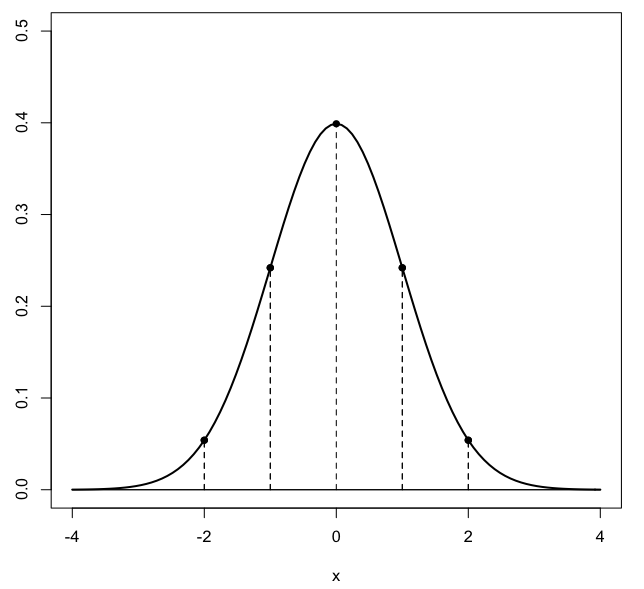
\includegraphics [scale=0.4] {gauss3.png} \end{center}

\begin{document}
\maketitle
\Large
\subsection*{visualization}

An electric (or gravitational) field at a point can be defined as the force that would be felt by a unit charge (or mass) placed at that point.  So for example
\[ \mathbf{F} = q \mathbf{E} \]

Fields, like forces are vectors.  That means, to every point in space there corresponds a vector with the magnitude and direction of the field or the force at that point.

Fields are often visualized by drawing lots of little arrows.  For example, here is a representation of the magnetic field surrounding a magnet:

\begin{center} 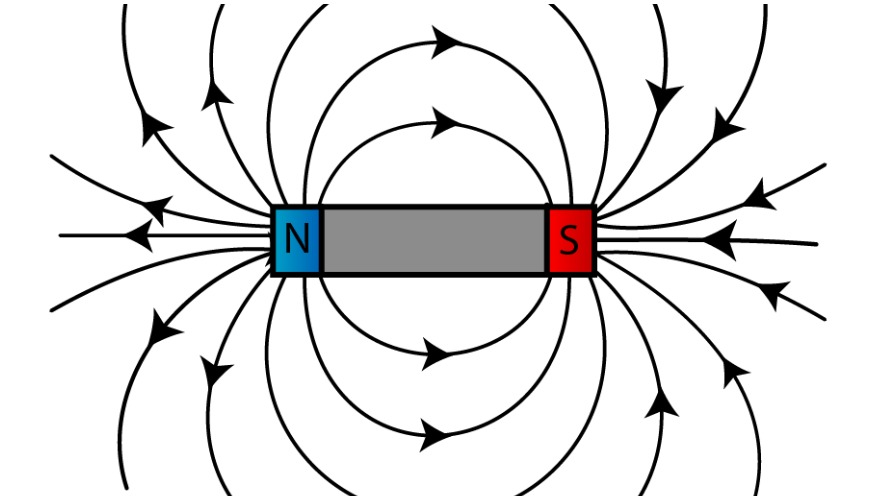
\includegraphics [scale=0.3] {magnet1.jpg} \end{center}

A classic physical demonstration of this field is obtained by overlaying the magnet with a sheet of paper and then sprinkling iron filings (small thin pieces) on top.  

\begin{center} 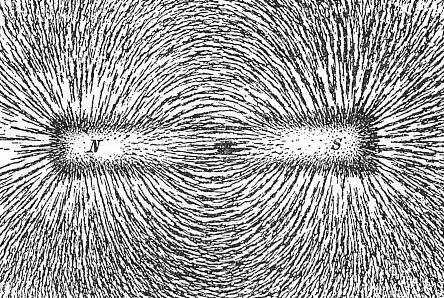
\includegraphics [scale=0.5] {magnet2.png} \end{center}

The filings align with the field, and tend to line up head-to-tail.  The field also exists between the lines of filings, but this looks something like the vector field one draws with arrows.

\subsection*{vector fields}
In two dimensions, vector field assigns to every point $(x,y)$ in a region $R$ in the plane a vector $\mathbf{F}(x,y)$ with two components
\[ \mathbf{F}(x,y) = M(x,y) \mathbf{i} + N(x,y) \mathbf{i} \]

Each of the component functions $M$ and $N$ takes an ordered pair of real numbers and outputs a real number.  As a shorthand, we could write:
\[ \mathbf{F} = \langle M, N \rangle \]

In three dimensions we might have $\mathbf{F} = \langle P, Q, R \rangle$.  We could also write the components of $\mathbf{F}$ explicitly as some functions of $x$ and $y$, e.g.
\[ \mathbf{R} = \langle x,y \rangle \]

This is the field of radial vectors, all of which point in the direction opposite to the origin, and have length $r = \sqrt{x^2 + r^2}$.  We could also normalize to get $\mathbf{R}/r$ or even $\mathbf{R}/r^2$.

The spin field is $\mathbf{S} = \langle -y,x \rangle$.  These can be normalized or divided by $r^2$ as for $\mathbf{R}$.

\subsection*{potential}

A \emph{gradient field} is the gradient of some function $f$ which is called the potential.  Such fields are conservative, as we'll see later on.  Recall that the gradient is
\[ \nabla f = \langle f_x, f_y \rangle \]
where by $f_x$ I mean the $x$-derivative of $f$.  The radial fields are all gradient fields.  Consider
\[ f(x,y) = \frac{1}{2}(x^2 + y^2) \]
Clearly
\[ \nabla f = \langle x, y \rangle = \mathbf{R} \]
The gradient is everywhere perpendicular to the level curves $f(x,y) = c$.

Some fields are gradient fields, and some are not.

What is the potential function for 
\[ \frac{\mathbf{R}}{r} = \frac{1}{\sqrt{x^2 + y^2}} \  \langle x,y \rangle \]

Well, what function $f$ has as its $x$-derivative $x/\sqrt{x^2 + y^2}$?
\[ \frac{\partial}{\partial x} \  \sqrt{x^2 + y^2} =  \ ?\]
That looks right.



\end{document} 